% !TeX root = ../dissertation.tex
\section{Motivation}
\label{sec:motivation}

\begin{figure}[!th]
	\centering
	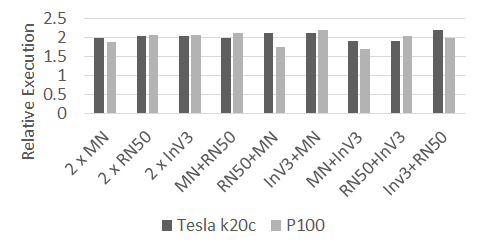
\includegraphics[width=.9\columnwidth]{images/shared-training.png}
	\caption{{\footnotesize Three TensorFlow workloads sharing an NVIDIA Tesla GPU. \aak{Apologies for being brutal, but this is pretty weak sauce. The data is noisy/inconclusive at best. I understand the reason to have this graph, but unless we can draw out some patterns (e.g. combinations that under-utilize the K20c should have much worse under-utilization on the p100 --- that shows that the problem is getting worse.) from the graph, it's hard to see any signal here.}}}
	\label{fig:motivation}
\end{figure}

\textbf{Fallacy:} \emph{most GPU workloads can fully utilize a GPU.}
This is a common misconception that is often touted to justify
the use of techniques that \emph{expose} dedicated GPU hardware~\cite{AWS-gpu}
rather than \emph{virtualize} them.
% to enable sharing it across protection domains.
On the contrary, the compute density of GPUs continues to grow at a pace
that suggests that it is almost certain that under-utilization of GPU
resources will be a major pain-point for cloud providers in the future, if it
already isn't.

To illustrate the opportunity, we co-scheduled three TensorFlow~\cite{
abadi2016tensorflow} programs --- MobileNet, ResNet50, InceptionV3 --- in
pairs, on a single NVIDIA Tesla~\cjr{TODO get machine
details} GPU~\footnote{Execution times for all the programs are on the order of hundreds of seconds. The batch size was 32. The \texttt{allow\_growth}
option was enabled to prevent TensorFlow from pre-allocating all GPU
memory and \texttt{gpu\_memory\_fraction} was set to 0.5 in GPUOptions to
ensure at most half of the GPU memory is used for each co-scheduled program.}, and measured the execution (inference) time.
% , all from TensorFlow's \texttt{tf.keras.applicat\-ions},

Figure~\ref{fig:motivation} shows the relative execution time of all possible
co-schedules of these workloads. Considering their total serial execution time
on dedicated hardware to be 2$\times$, cases where relative times exceed
2$\times$ indicate slowdown due to contention; those that are under 2$\times$
indicate under-utilization. Under-utilization of GPU resources indicates a
failure to fully leverage the hardware (e.g. by co-scheduling GPU kernels with
complementary resource demands). While slowdown from contention does occur (at
most 10\% of total serial execution time), \( \frac{4}{9} \) of the cases
yield \emph{speedup}. The data are evidence that the cost of sharing is
tolerable and under-utilization is real. Our findings are corroborated by
others~\cite{long-list-of-citations-hangchen-dug-up}. We note that newer GPU
hardware, such as NVIDIA Volta V100~\cite{volta-nvidiaweb}, have many times
the compute density of the GPUs we tested, and the growth trend is projected
to continue.